%%%%%%%%%%%%%%%%%%%%%%%%%%%%%%%%%%%%
\chapter{Literature Review} 
\label{chap:Literature_Review}
%%%%%%%%%%%%%%%%%%%%%%%%%%%%%%%%%%%%
\comment{
Use your literature review to help the reader to understand the value and the interest in your project.  You should look for related works already published that either support the merit of your project, or provide the background understanding/information to make your new claims.  Try to avoid writing a "catalogue" of related works (e.g this would have little of your own insight added).  Instead, describe to the reader why the related work is interesting or relevant to your own work.  What did they achieve?  What did they overlook?  It is highly recommend you finish your Literature Review with a final subsection "Summary", where you may wish to formulate highly specified research questions or hypotheses, or assert the need for your Research Methodology (next chapter).  

introduction
literature review
implementation
research methodology
results




\section{This is a section}
\subsection{This is a subsection}
\subsubsection{This is subsubsection}

%%%%%%%%%%%%%%%%%%%%%%%%%%%%%%%%%%%%
% Figure with subfigures
%%%%%%%%%%%%%%%%%%%%%%%%%%%%%%%%%%%%

\begin{figure}[htb]
\centering
\begin{subfigure}[t]{.5\textwidth}
  \centering
  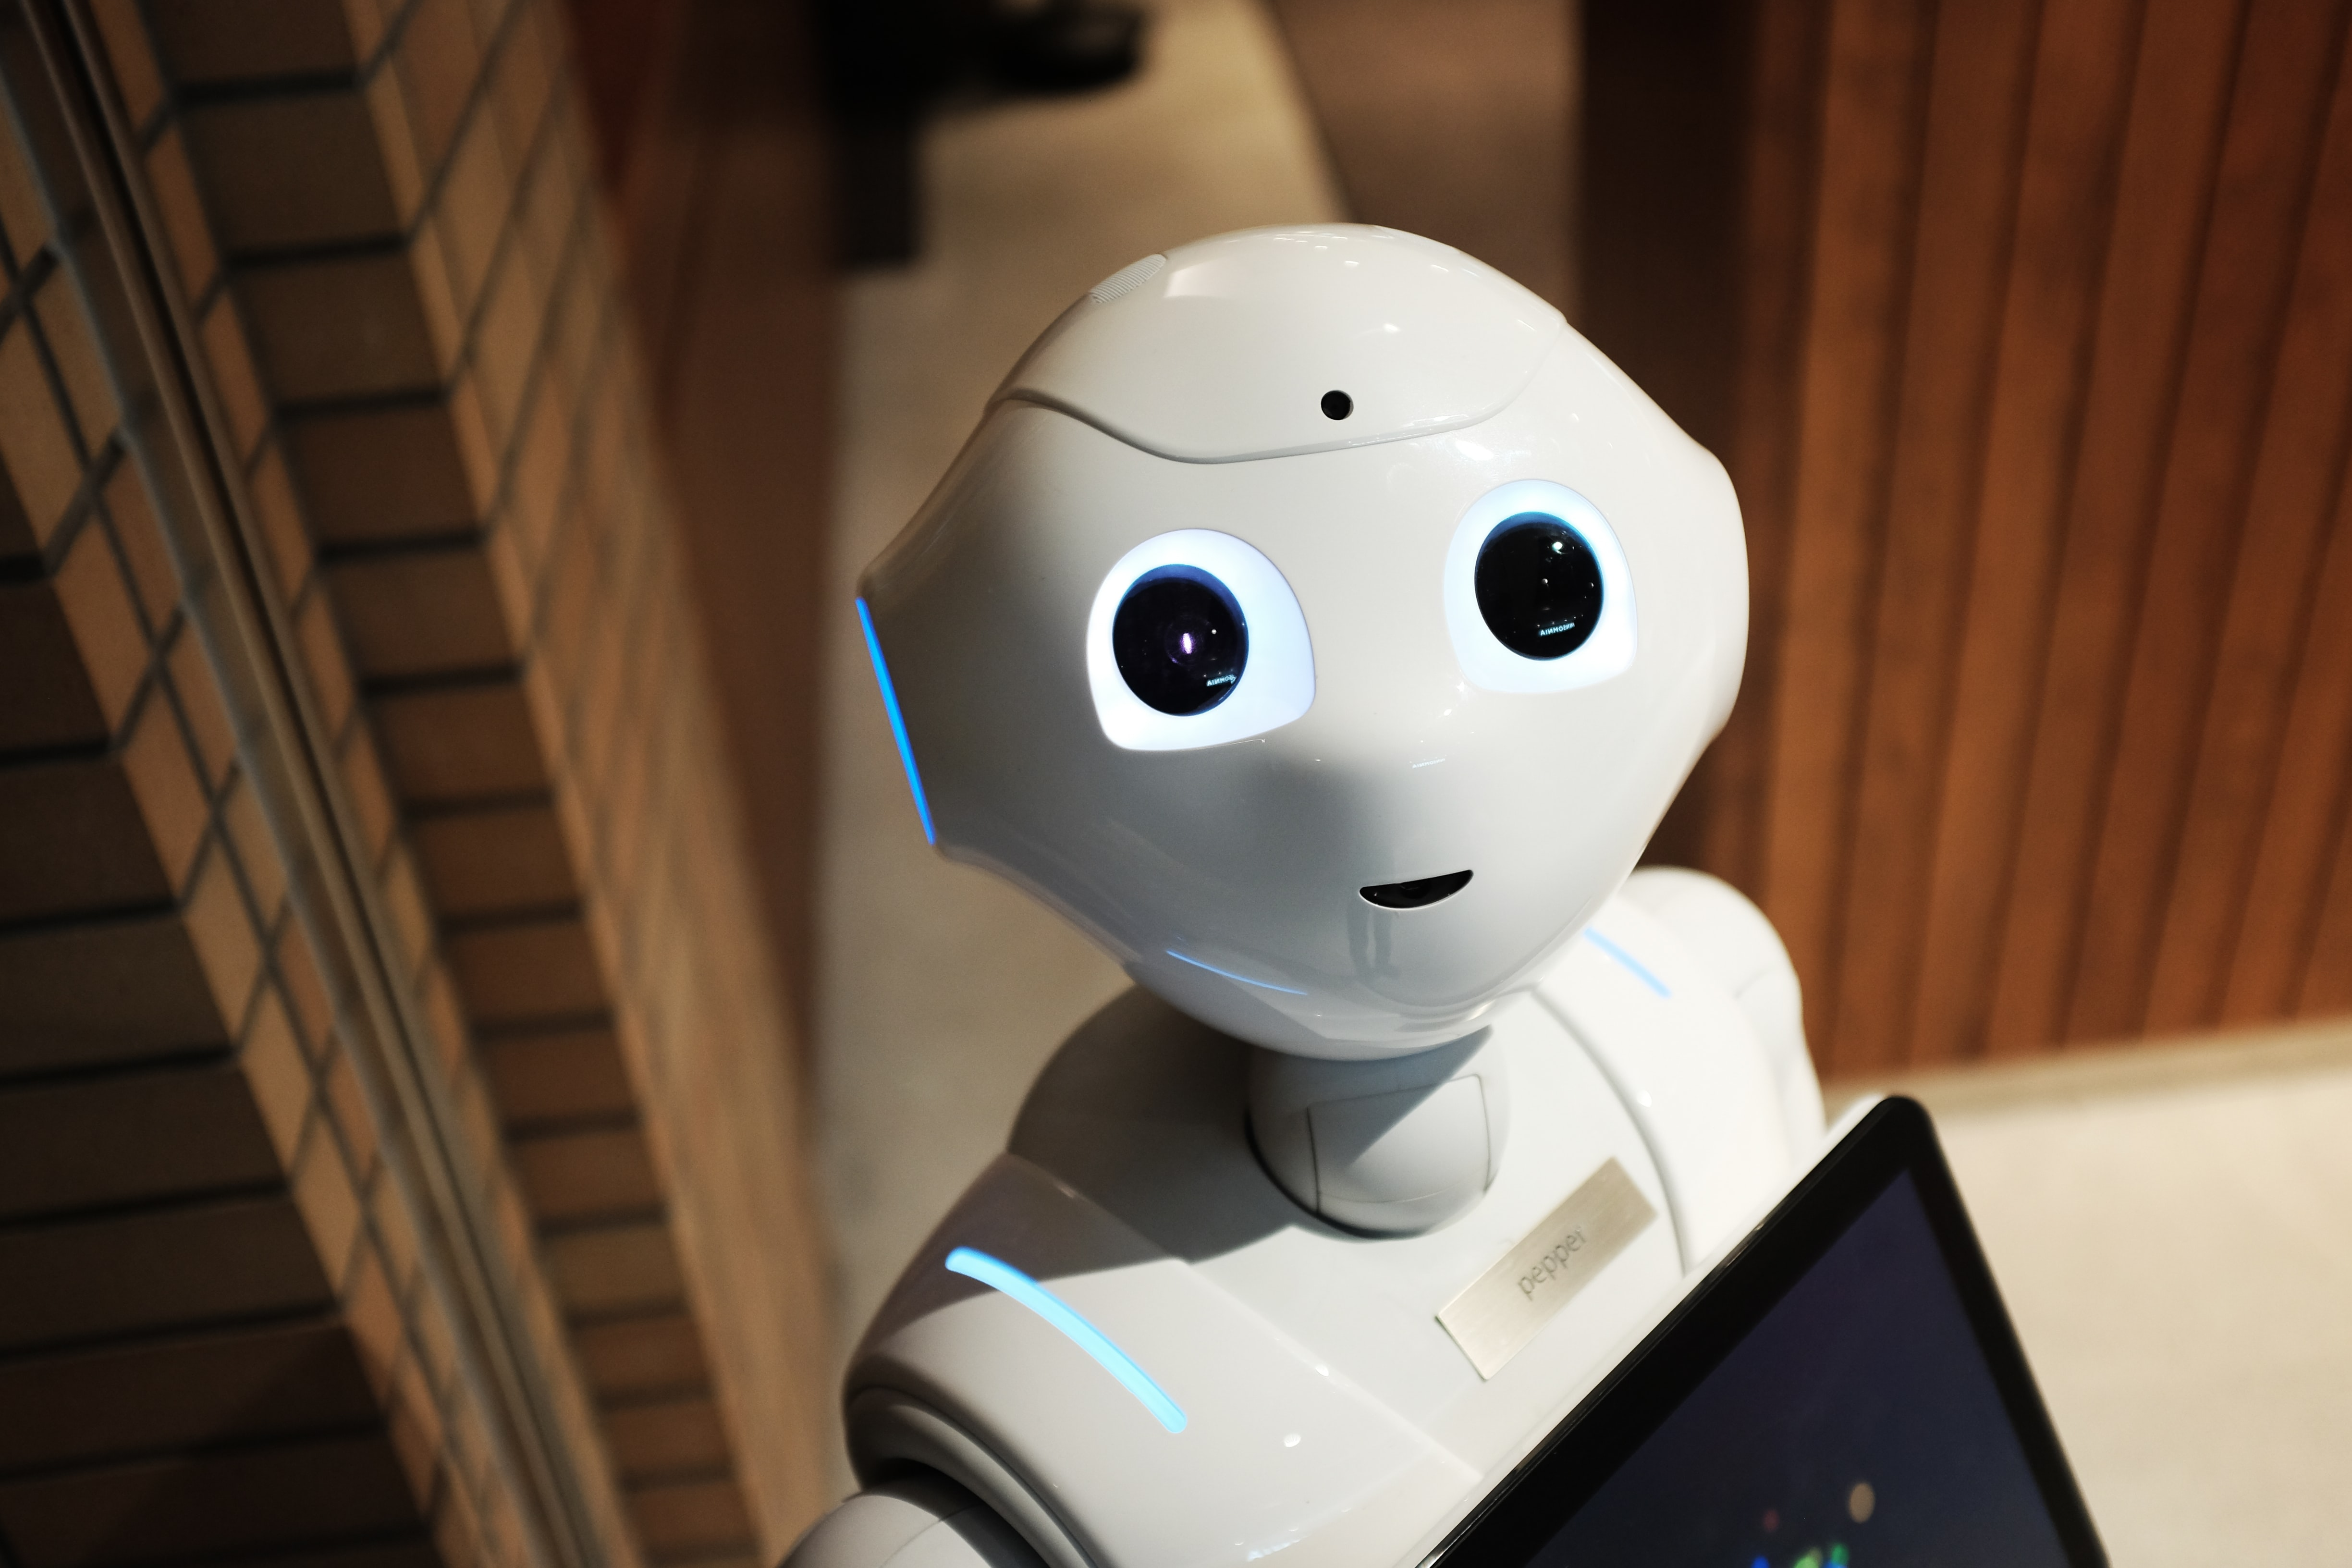
\includegraphics[height=4.5cm]{figures/Robot_1.jpg}
  \caption{\label{fig:left_robot} This is a robot.}
  \label{fig:theoretical}
\end{subfigure}%
\begin{subfigure}[t]{.5\textwidth}
  \centering
  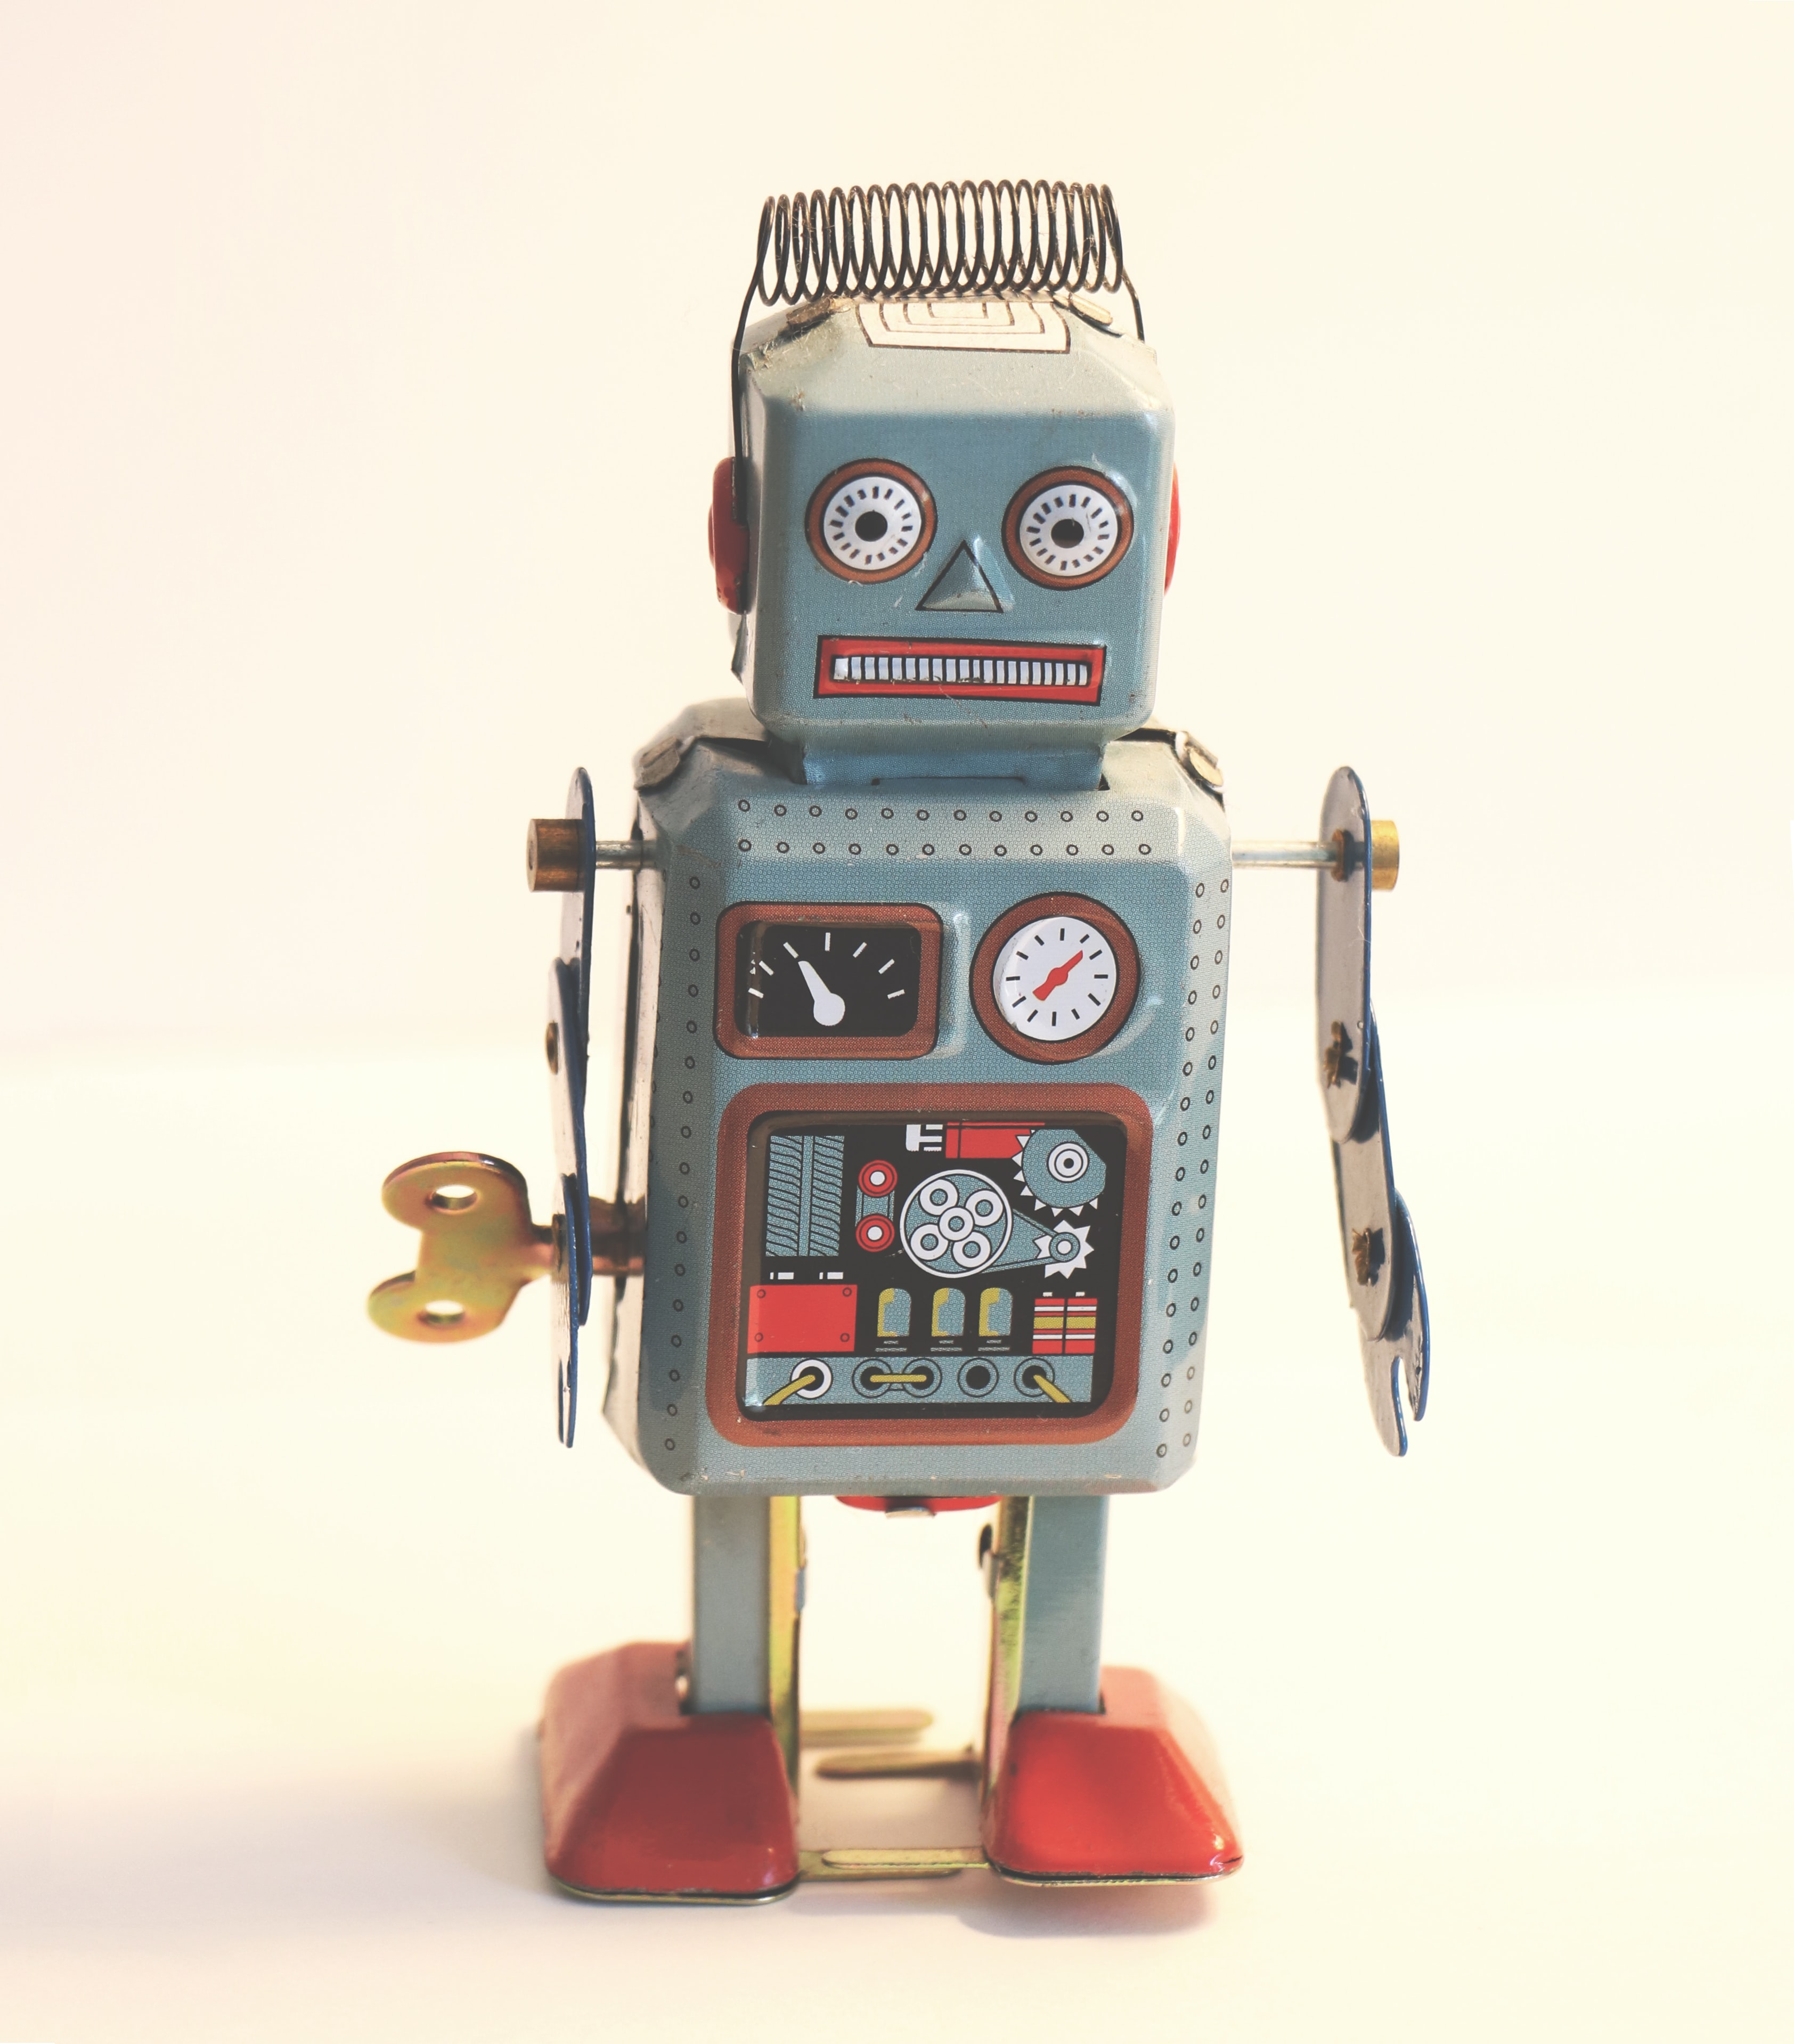
\includegraphics[height=4.5cm]{figures/Robot_2.jpg}
  \caption{\label{fig:right_robot} This another robot.}
  \label{fig:practical}
\end{subfigure}
\caption{\label{fig:two_robots} These are two robots}
\label{fig:test}
\end{figure}

For example, \cite{Robots2020} discusses the two robots depicted in Figure \ref{fig:two_robots}. There is a robot in Figure \ref{fig:left_robot} and another robot in Figure \ref{fig:right_robot}.

}

This section will provide the details of the STDMA\cite{STDMA} protocol and a review of the related \textit{Distributed Model Predictive Control} (DMPC) algorithms.

\section{STDMA Explained}

As previously mentioned in Section \ref{chap:Brief Introduction}, STDMA stands for \textbf{\textit{Self-organised Time-Divided Multiple Access}}, and it allows multiple agents to share the same channel for communication without centralised control.
The main assumtion of this protocol is that all agents have synchronised clocks. In practice, this is achieved through GPS\cite{STDMA_GPS}.

\textbf{The core idea of STDMA could be summarised as follows}: Represent continuous time with repeating frames that are consisted of discrete time slots.
While agents are always listening to messages from the channel, they look for free slots to occupy, and therefore use the occupied slots to broadcast their own data.

Agents using STDMA have \textbf{four phases}, which are arranged in chronological order as follows:

\begin{enumerate}
  \item \textbf{Initialisation}: Agents in this phase have not yet joined the network. The device listens to an entire frame and determines current allocation of each slot.
  \item \textbf{Network Entry}: Randomly choose an unallocated slot to broadcast their existance and reserve one slot for the next phase.  If the message sent didn't collide with others (i.e., only one agent which is myself choose to use this slot for entering), then the entering is successful. If the entering failed, reverse to the previous phase.
  \item \textbf{First Frame}: Use the slot reserved in the previous phase to reserve more slots for themselves. The number of reserved slots depends on the size of the data packet that the agent needs to send in each frame.
  \item \textbf{Continuous Operation}: Use the previously reserved slots to work normally. If some slots are released or more slots are needed, reapply for slots.
\end{enumerate}

Although the description above omitted some details (such as slot choosing strategy, calculation of required number of slots, etc.), it is clear that \textbf{the core idea of STDMA is the strategy of finding and reserving unallocated slots}.

This protocol also has several limitations, such as: \textbf{(1)} Collision in entering: In the Network Entry phase, multiple agents may accidentally choose the same unallocated slot for entering and broadcast their existance. \textbf{(2)} Capacity: When slots are not enough, conflicts would inevitably occur. 
There are some studies \cite{STDMA_improv1,STDMA_improv2} that proposed improvements for its limitations, but improving STDMA is not the focus of this project.

For detailed implementation, please see \textbf{PLACEHOLDER}.

\section{Distributed Model Predictive Control}

This section would cover:
\begin{itemize}
  \item An brief introduction to DMPC.
  \item Why is DMPC related to this project.
  \item A summary of related latest research developments.
\end{itemize}

\subsection{Brief Introduction}
\subsubsection{What is Model Predictive Control\cite{MPC_Review1}?}

\textit{Model Predictive Control} or MPC is a form of control that based on the model and the online prediction of the controlled system.

MPC achieves its control objective by optimising the predicted outcome of the model of the controlled system\cite{MPC_Review1}.
\textbf{On every sampling instant}, a typical MPC controller would \textbf{use the current state of the plant as initial state}, and \textbf{solve a finite-horizon open-loop optimal control problem in real-time speed}, then \textbf{apply the first step of the generated control sequence} as the next control action.

The major challenge confronting the MPC algorithm is the stability issue, with several factors contributing to this problem, such as inadequate terminal conditions and limited prediction horizons.

MPC has been extensively studied and is a widely used control algorithm\cite{DMPC_Review1}. 
It's primarily employed in fields such as process industry, power electronics, building climate and energy management, and manufacturing\cite{MPC_Applications1, MPC_Applications2}.

\subsubsection{What is Distributed Model Predictive Control? \cite{DMPC_made_easy}}

% 当系统的规模达到一定大小的时候,单一的中心化MPC控制器就不能完成控制任务了(计算要求过高/只能向有限的邻居发送数据等)。所以需要DMPC:


In many scenarios, centralised controllers fail to perform control tasks due to reasons such as the computational load increasing with the expansion of system scale, 
resulting in the controller's inability to complete real-time computations, 
or the inability to dispatch control information to all components of the system within a specified time. 
In summary, \textbf{the limitations of centralised controllers made them incapable of meeting the needs of many control scenarios}, and that is why we need distributed control.

For \textit{Distributed Model Predictive Control} or DMPC, a large system is decomposed to numerous subsystems, and each of them:
\begin{itemize}
  \item Has its own dynamic.
  \item Has an MPC controller to control its actions (predict finite future states and choose the optimal current move).
  \item Could interact with and be influenced by other subsystems (usually described as \textit{variables} and \textit{constraints}).
\end{itemize}


DMPC algorithms have the following \textbf{key characteristics}, which can help readers to understand the algorithms and distinguish one algorithm from another:

\begin{itemize}
  \item \textbf{Architecture}: Different relationships between local MPC controllers. \textbf{Hierarchical}: The entire system is divided into layers, each containing several subsystems with MPC controllers, and there exists a hierarchical relationship between these layers. \textbf{Decentralised}: Each local MPC controller controls the local subsystem and don't communicate with each other. \textbf{Distributed}: Local MPC controllers cooperate to find better solution for the overall system.   
  \item \textbf{Local - Global}: How much do the local controllers know about the overall system information.
  \item \textbf{Selfish - Cooperative}: Whether the local controller only optimizes its own cost.
  \item \textbf{Iterative - Non-Iterative}: Whether the control strategy is generated through exchange and iteration among multiple local controllers.
  \item \textbf{Serial - Parallel}: Whether the local controllers transmit their messages in a specific order or multiple controllers could communicate with each other at the same time.
  \item \textbf{Synchronised - Asynchronised}: Whether the local controllers follow a shared schedule for computation and communication. 
\end{itemize}

The advantages and disadvantages of DMPC both stem from its decentralised nature. 
Like many other decentralised algorithms, \textbf{DMPC has better scalability and robustness}, can bypass communication bottlenecks, and to some extent, allows for parallel processing.
But \textbf{coordination among multiple controllers can be quite complex},
e.g., all local controllers tend to achieve Nash equilibrium for themselves, but such a tendency may not contribute to reaching Pareto optimality and might even be counterproductive for the entire system\cite{Nash_Equi}.

\subsubsection{Why is this project related to DMPC?}

The designed algorithm (detailed explanation please see Section \textbf{PLACEHOLDER}) in this project allows each agent to:
\begin{itemize}
  \item Create and join a self-organised serial communication channel.
  \item Determine the time window for planning and plan broadcasting.
  \item Use the shared channel to broadcast its own moving plan.
  \item Receive plans of other agents and use the received information to its own movement.
\end{itemize}

Which means, the presented algorithm could be classified as a DMPC algorithm, and the problem it solves could be treated as a DMPC problem.

\subsection{Latest Researches of DMPC}


